%-----------------------------------------------------------------------
%\subsection{Mode and Level}
%-----------------------------------------------------------------------
%\tbc
%Baseliyos Jacob
\textbf{This paragraphs gives an overview about the input documents used for the:}
\begin{itemize}
\item Analysis of the OBU Functions
\item Functional decomposition and allocation of functional blocks, functions and libraries.
\item Design of the OBU Functions
\item Determination of "Use Cases" and Scenarios for the different iteration of the Architecture and Design Document
\end{itemize} 

\textbf{List of main documents that are being used as reference or input for analysis and design:}

\begin{itemize}
\item\textbf{ERA TSI CCS Documents}
\item\textbf{openETCS API Spec}
\item\textbf{openETCS Requirements WP 2}
\item\textbf{Railway Operator Documents}
\item\textbf{Industry Documents}
\item\textbf{ERSA Simulator Documents}
\item\textbf{Other Project Partner Data information and documents}
\item\textbf{Utrecht - Amsterdam Track Documents}
\end{itemize}

\textbf{Furthermore relevant ETCS Know How from Industry and Operator is used for the design and the analysis}

\textbf{While the list above serves as high- level reference, detailed information, links to the actual documents and additional remarks are being maintained at:}
\url{https://github.com/openETCS/modeling/wiki/Input-Documents-Repository}
while the documents describing the standard are referenced here: \url{https://github.com/openETCS/SSRS/wiki/SSRS-Documents}

The figure below illustrates  the relationships among the input used documents: \

\begin{figure}[h]
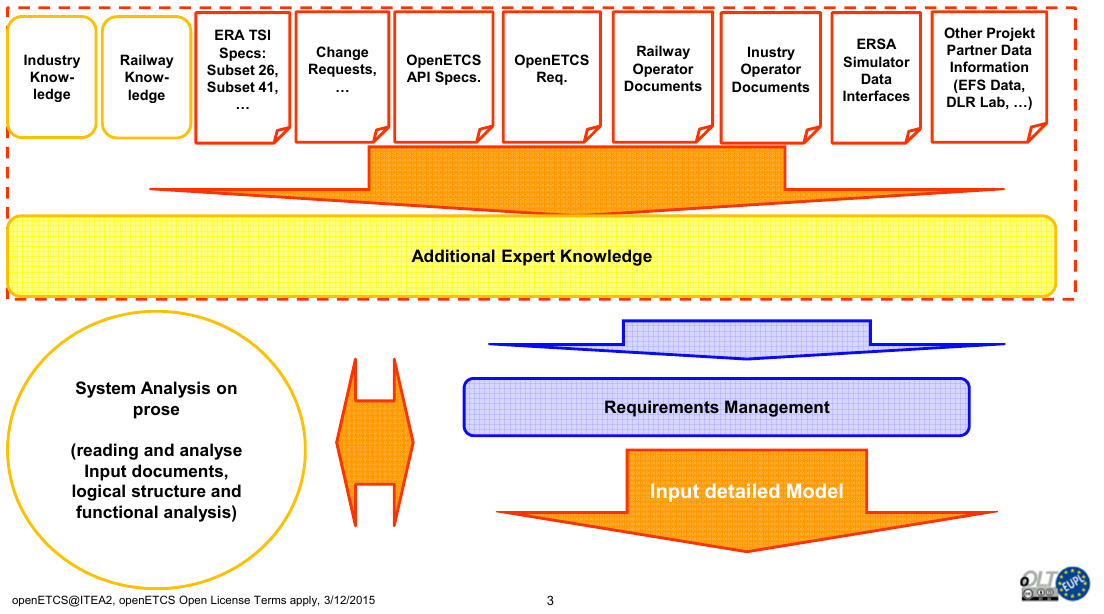
\includegraphics[scale=0.5]{images/AnalysisDocuments}
\caption{Analysing of input document}
\label{Analyising of input document}
\end{figure}

For a detailed discussion of the actual work process, please refer to the previous chapters. 

